\begin{frame}{Interne datoteke}
	\begin{itemize}
		\item{Git unutar .git direktorija svakog repozitorija sprema datoteke koje sadrže informacije o repozitoriju}
		\item{Neke od tih informacija su popis grana, promjene spremljene u index, konfiguracija, lokacija HEAD-a i sl.}
		\item{Git svim commitovima i podacima pridodaje jedinstvene ključeve (hasheve) koji se koriste za identificiranje i pristup tim podacima i koriste se u internim gitovim datotekama}
	\end{itemize}
\end{frame}
\begin{frame}{Datoteka config}
	\begin{itemize}
		\item{Datoteka config unutar .git direktorija sadrži osnovne podatke o repozitoriju kao što je popis svih povezanih udaljenih repozitorija, poveznicu na master granu zadanog default repozitorija i interne opcije kao što je osjetljivost na velika i mala slova}
		\item{Primjer config datoteke:}
	\end{itemize}
	\begin{center}
		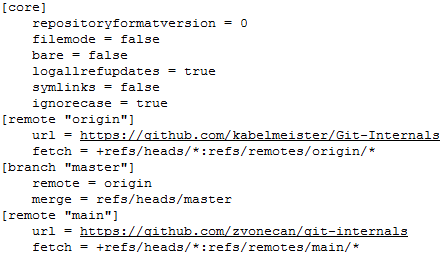
\includegraphics[width=0.66\linewidth]{img/config.png}
	\end{center}
\end{frame}
\begin{frame}{Datoteke HEAD i FETCH\_HEAD}
	\begin{itemize}
		\item{Datoteka HEAD sadrži referencu na trenutno checkoutan commit ili granu}
		\item{Ako je checkoutan commit onda datoteka sadrži jedinstveni hash tog commita (npr. 0e9dc3b589624f744f06b34450829382a61bfe44)}
		\item{U slučaju da je checkoutana neka grana onda datoteka sadrži referencu do te grane u obliku: ref: refs/heads/<grana>}
		\item{Datoteka FETCH\_HEAD sadrži jedinstveni hash commita kad je zadnji put napravljen fetch sa udaljenog repozitorija te ime grane i lokaciju udaljenog repozitorija}
	\end{itemize}
\end{frame}
\begin{frame}{Direktorij refs/}
	\begin{itemize}
		\item{Direktorij refs sadrži sadrži poddirektorije heads, remotes i tags te datoteku stash koja sadrži hash privremenog commita sa stashanim promjenama}
		\item{Direktorij refs/heads sadrži datoteku za svaku granu u repozitoriju u kojima je zapisan hash zadnjeg commita u pojedinoj grani}
		\item{Sličan direktoriju refs/heads, refs/remotes razlikuje se po tome što su u njemu zapisani isti podaci, ali za sve povezane udaljene repozitorije}
		\item{Unutar direktorija refs/tags nalaze se datoteke sa svim tagovima koji se koriste u repozitoriju a u njima je zapisan hash commita koji je tagiran tim tagovima}
	\end{itemize}
\end{frame}